\documentclass[12pt]{article}

\usepackage[utf8]{inputenc}
\usepackage{latexsym,amsfonts,amssymb,amsthm,amsmath,graphicx,mathtools,subfig,hyperref,float,bm}
\usepackage[parfill]{parskip}
\usepackage[export]{adjustbox}
\usepackage[justification=centering]{caption}
\usepackage{nameref}
\usepackage{cleveref}

\hypersetup{
    colorlinks=true,
    linkcolor=blue,
    filecolor=magenta,      
    urlcolor=cyan,
}

\DeclareMathAlphabet{\mymathbb}{U}{BOONDOX-ds}{m}{n}

\setlength{\parindent}{0in}
\setlength{\oddsidemargin}{0in}
\setlength{\textwidth}{17cm}
\setlength{\textheight}{22cm}
\setlength{\topmargin}{0cm}
\setlength{\headheight}{0pt}
\setlength{\footskip}{30pt}

\DeclareMathOperator*{\argmax}{arg\,max}
\DeclareMathOperator*{\argmin}{arg\,min}
\DeclareMathOperator*{\lmo}{lmo}
\DeclareMathOperator*{\tr}{Tr}


\renewcommand{\thesubsubsection}{\thesubsection.\alph{subsubsection}}

\newcommand{\boldZ}{\mathbf{Z}}
\newcommand{\boldX}{\mathbf{X}}
\newcommand{\boldU}{\mathbf{U}}
\newcommand{\boldV}{\mathbf{V}}
\newcommand{\setX}{\mathcal{X}}
\newcommand{\boldS}{\mathbf{\Sigma}}
\newcommand{\boldu}{\mathbf{u}}
\newcommand{\boldv}{\mathbf{v}}
\newcommand{\boldb}{\mathbf{b}}
\newcommand{\boldA}{\mathbf{A}}
\newcommand{\boldC}{\mathbf{C}}
\newcommand{\boldOne}{\mathbf{1}}
\newcommand{\dist}{\text{dist}}
\newcommand{\QP}{\text{QP}}
\newcommand*{\proj}{\text{proj}}

\title{EE-556 Homework 4}
\author{Edoardo Debenedetti}

\begin{document}

\maketitle

\section{Theory: Projection free convex low-rank matrix optimization}

\subsection{Projection onto the nuclear norm ball}
\subsubsection{Projection proof}
\begin{proof}
Let $\boldZ = \boldU\boldS\boldV^T$ be the SVD of $\boldZ \in \mathbb{R}^{p \times m}$, and $\setX = \{ \boldX : \lVert \boldX \rVert_{*} \leq \kappa \}$, we can write the projection of $\boldZ$ onto $\setX$ as:
\begin{equation}
    \proj_{\setX}(\boldZ) = \argmin_{\boldX \in \setX} \lVert \boldX - \boldZ \rVert_{F}
\end{equation}

Let us first look for the projection, onto $\setX$ of $\boldS$:
\begin{equation}
    \proj_{\setX}(\boldS_{\boldZ}) = \argmin_{\boldS_{\boldX} \in \setX} \lVert \boldS_{\boldX} - \boldS_{\boldZ} \rVert_{F}
\end{equation}
However, given that $\boldS$ is diagonal, its nuclear norm $\lVert \boldS \rVert_{*}$ is the sum of its singular values. However, as $\Sigma$ is diagonal, its singular values are given by the diagonal itself, and their sum is the sum of the diagonal elements. Moreover, its diagonal elements are the only non-zero elements, and then, when computing its $\ell1$-norm $\lVert \boldS \rVert_{1}$, we sum only the absolute value of the diagonal. Moreover, as the entries of $\boldS$ are singular values, they are all non-negative and they are equal to their absolute value. Hence, $\lVert \boldS \rVert_{*} = \lVert \boldS \rVert_{1}$, and, when considering $\boldS$, $\setX = \{ \boldX : \lVert \boldX \rVert_{*} \leq \kappa \} = \{ \boldX : \lVert \boldX \rVert_{1} \leq \kappa \}$. Hence,
\begin{equation}
     \proj_{\setX}(\boldS_{\boldZ}) = \argmin_{\boldS_{\boldX} \in \setX} \lVert \boldS_{\boldX} - \boldS_{\boldZ} \rVert_{F} = \boldS_{\boldZ}^{\ell1}
\end{equation}
where $\boldS_{\boldZ}^{\ell1}$ is the projection of $\boldS_{\boldZ}$ onto the $\ell1$-norm ball smaller than $\kappa$. Moreover, we can state that
\begin{equation}
    \min_{\boldS_{\boldX} \in \setX} \lVert \boldS_{\boldX} - \boldS_{\boldZ} \rVert_{F} = \lVert \boldS_{\boldZ}^{\ell1} - \boldS_{\boldZ} \rVert_{F} \label{eq:sigma-proj}    
\end{equation}
Now let us consider, again, $\lVert \boldX - \boldZ \rVert_{F}$. Thanks to Mirsky's inequality we know that $\lVert \boldX - \boldZ \rVert_{F} \geq \lVert \boldS_{\boldX} - \boldS_{\boldZ} \rVert_{F}$, and then, thanks to \Cref{eq:sigma-proj}, we can state that $\lVert \boldX - \boldZ \rVert_{F} \geq \lVert \boldS_{\boldZ}^{\ell1} - \boldS_{\boldZ} \rVert_{F}$, which means that $\lVert \boldS_{\boldZ}^{\ell1} - \boldS_{\boldZ} \rVert_{F}$ is a lower bound for the projection argument.

If we set $\boldX = \boldU \boldS_{\boldZ}^{\ell1} \boldV^T$, we then have
\begin{gather}
    \lVert \boldU \boldS_{\boldZ}^{\ell1} \boldV^T - \boldU \boldS \boldV^T \rVert = \\
    = \lVert \boldU (\boldS_{\boldZ}^{\ell1} \boldV^T - \boldS \boldV^T) \rVert = \\
    = \lVert \boldU (\boldS_{\boldZ}^{\ell1} - \boldS) \boldV^T \rVert = \label{eq:frob-invariance-1} \\
    = \lVert \boldS_{\boldZ}^{\ell1} - \boldS \rVert \label{eq:frob-invariance-2}
\end{gather}

It is worth noting that between \Cref{eq:frob-invariance-1} and \Cref{eq:frob-invariance-2} we exploted the fact that $\boldU$ and $\boldV$ are unitary matrices and hence orthogonal, and that Frobenius norm is invariant of orthogonal matrices.

We can now note that if we set $\boldX$ as we did above, we get a norm which is equal to a lower-bound, and hence is a minimum, which means that
\begin{equation}
    \boldX = \boldU \boldS_{\boldZ}^{\ell1} \boldV^T \in \argmin_{\boldX \in \setX} \lVert \boldX - \boldZ \rVert_{F} = \proj_{\setX}(\boldZ)
\end{equation}
\end{proof}

\subsubsection{Implementation}
We can observe from \Cref{tab:projections} that the average duration with 1M entries matrix is exponentially larger than that with 100k entries. This is coherent with SVD decomposition complexity, which is exponential: $\mathcal{O}(\min(m^2p, mp^2))$.

\begin{table}[ht]
\centering
\caption{Duration of matrix projections onto the nuclear norm ball with $\kappa = 5000$.}
\label{tab:projections}
\begin{tabular}{ccccccc}
Measure & 1 & 2 & 3 & 4 & 5 & Average \\ \hline
100k (s) & 0.7198 & 0.6789 & 0.6661 & 0.677 & 0.6504 & 0.67844 \\ \hline
1M (s) & 37.6 & 35.4 & 35.42 & 35.27 & 35.25 & 35.788
\end{tabular}
\end{table}

\subsection{LMO of nuclear norm}
\subsubsection{LMO proof}
Given that
\begin{equation}
    \lmo_{\setX}(\boldZ) = \argmin_{\boldX \in \setX} \langle \boldX, \boldZ \rangle
\end{equation}
where $\langle \boldX, \boldZ \rangle = \tr(\boldZ^T\boldX)$, we want to show that
\begin{equation}
    -\kappa \boldu \boldv^T \in \lmo_{\setX}(\boldZ)
\end{equation}
As $\kappa \boldu \boldv^T \in \setX$, we just need to show that $\langle \boldX, \boldZ \rangle \geq \langle -\kappa \boldu \boldv^T, \boldZ \rangle$.

\begin{proof}
First, let us work on $\langle -\kappa \boldu \boldv^T, \boldZ \rangle$:
\begin{gather}
    \langle \kappa \boldu \boldv^T, \boldZ \rangle = \tr(\boldZ^T (-\kappa \boldu \boldv^T)) = \\
    = -\kappa \tr(\boldZ^T \boldu \boldv^T)
\end{gather}
Thanks to variational characterization of singular vectors, $\boldZ^T \boldu = \sigma \boldv$, where $\sigma$ is the singular value corresponding to the singular vectors $\boldu$ and $\boldv$, i.e. the largest singular value. Hence we get
\begin{gather}
    \langle \kappa \boldu \boldv^T, \boldZ \rangle = -\kappa \tr(\sigma \boldv \boldv^T) = \\
    = -\kappa \sigma \tr(\boldv \boldv^T) = -\kappa \sigma \label{eq:inner-kuv-z}
\end{gather}
Where we leveraged the fact that $\boldv$ is a column of the unitary matrix $\boldV$ and then its inner product with itself $\langle \boldv, \boldv \rangle = \tr(\boldv^T\boldv) = \tr(\boldv\boldv^T) = 1$.

If we now take in consideration $\langle \boldX, \boldZ \rangle$, we know that, thanks to H{\"o}lder's inequality
\begin{equation}
    \lvert \langle \boldX, \boldZ \rangle \rvert \leq \lVert \boldX \rVert_{q} \cdot \lVert \boldZ \rVert_{r}, \ \ r > 1, \ \frac{1}{q} + \frac{1}{r} = 1
\end{equation}
If we choose the nuclear norm for $\boldX$ and the infinity norm for $\boldZ$, then $q = 1$ and $r = \infty$, and $\frac{1}{q} + \frac{1}{r} = 1$. Then we have that
\begin{equation}
    \lvert \langle \boldX, \boldZ \rangle \rvert \leq \lVert \boldX \rVert_{*} \cdot \lVert \boldZ \rVert_{\infty}
\end{equation}
Removing the absolute value we obtain
\begin{equation}
    \langle \boldX, \boldZ \rangle \geq - \lVert \boldX \rVert_{*} \cdot \lVert \boldZ \rVert_{\infty}
\end{equation}
Since, we need $\boldX \in \setX$, then $\lVert \boldX \rVert_{*} \leq \kappa$, which leads to $-\lVert \boldX \rVert_{*} \geq -\kappa$. Hence, $\lVert \boldX \rVert_{*} \cdot \lVert \boldZ \rVert_{\infty} \geq -\kappa \lVert \boldZ \rVert_{\infty}$, and we obtain
\begin{equation}
    \langle \boldX, \boldZ \rangle \geq \lVert \boldX \rVert_{*} \cdot \lVert \boldZ \rVert_{\infty} \geq -\kappa \lVert \boldZ \rVert_{\infty}
\end{equation}
Since $\lVert \boldZ \rVert_{\infty} = \sigma$, where $\sigma$ is the largest singular value of $\boldZ$, we can show that
\begin{equation} \label{eq:inner-x-z}
    \langle \boldX, \boldZ \rangle \geq - \kappa \sigma
\end{equation}
Finally combining \Cref{eq:inner-kuv-z} and \Cref{eq:inner-x-z}, we obtain
\begin{equation}
    \langle \boldX, \boldZ \rangle \geq - \kappa \sigma = \langle \kappa \boldu \boldv^T, \boldZ \rangle
\end{equation}
Hence
\begin{equation}
    \langle \boldX, \boldZ \rangle \geq \langle \kappa \boldu \boldv^T, \boldZ \rangle
\end{equation}
\end{proof}

\subsubsection{Implementation}
We can see from \Cref{tab:lmo-durations} that the duration with a 1M entries matrix is less than 10 times larger than the one with 100k entries, which is a significantly smaller ratio than that of projection.

\begin{table}[ht]
\centering
\caption{Duration of LMO computation with $\kappa = 5000.$}
\label{tab:lmo-durations}
\begin{tabular}{lllllll}
Measure & 1 & 2 & 3 & 4 & 5 & Average \\ \hline
100k & 0.1124 & 0.4546 & 0.0401 & 0.0539 & 0.0369 & 0.13958 \\ \hline
1M & 0.7298 & 1.227 & 1.14 & 1.001 & 0.2803 & 0.87562
\end{tabular}
\end{table}

\section{Hands-on experiment 1: Crime Scene Investigation with Blind Deconvolution}

\subsection{Frank-Wolfe for Blind Deconvolution}
\subsubsection{Objective function Lipschitz-smoothness}
\begin{proof}
We first compute the gradient of $f(\boldX) = \frac{1}{2} \lVert \boldA(\boldX) - \boldb \rVert_{2}^{2}$, where $\boldA$ is a linear operator and therefore can be treated as a matrix. The gradient is
\begin{equation}
    \nabla f(\boldX) = \nabla \frac{1}{2} \lVert \boldA(\boldX) - \boldb \rVert_{2}^{2} = \boldA^T(\boldA(\boldX) - \boldb)
\end{equation}
Then, in order to prove the Lipschitz smoothness of the gradient, we need to find a bounded $L$ such that
\begin{equation} \label{eq:lipschitz}
    \lVert \nabla f(\boldX_1) - \nabla f(\boldX_2) \rVert_{2} \leq L \lVert \boldX_1 - \boldX_2 \rVert_{2}
\end{equation}
Let us work on the first term:
\begin{gather}
    \lVert \nabla f(\boldX_1) - \nabla f(\boldX_2) \rVert_{2} = \lVert \boldA^T(\boldA(\boldX_1) - \boldb) - \boldA^T(\boldA(\boldX_2) - \boldb) \rVert_{2} = \\
    = \lVert \boldA^T(\boldA(\boldX_1) - \boldb - \boldA(\boldX_2) + \boldb) \rVert_{2} = \\
    = \lVert \boldA^T\boldA(\boldX_1 - \boldX_2) \rVert_{2} \leq
    \lVert \boldA^T\boldA \rVert_{2 \rightarrow 2} \cdot \lVert \boldX_1 - \boldX_2 \rVert_{2}
\end{gather}
Where we used Cauchy-Schwartz inequality. As $\lVert \boldA^T\boldA \rVert_{2 \rightarrow 2}$ is bounded, \Cref{eq:lipschitz} is satisfied.
\end{proof}

\subsection{Implementation}
As can be seen from \Cref{fig:plate}, the original plate number is \textit{J209 LTL}. The best result is obtained after just 30 iterations using $\kappa = 100$, and a $17 \times 17$ support. Using a smaller support leads to a too dark and indistinguishable picture, while a larger support can not run due to memory issues since with a larger support the matrices to work with become larger as well.

\begin{figure}[ht]
    \centering
    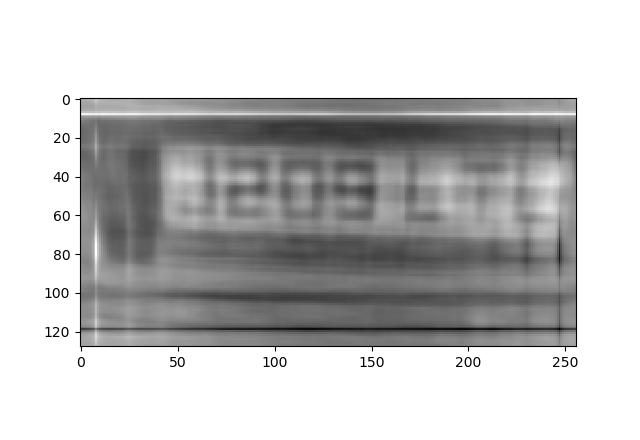
\includegraphics[width=17cm]{hw4/code/part2/results/100_30iters.png}
    \caption{Plate deblurring after 30 iterations using $\kappa = 100$}
    \label{fig:plate}
\end{figure}

\section{Hands-on experiment 2: k-means Clustering by Semidefinite Programming}

\subsection{Conditional Gradient Method for Clustering Fashion-MNIST data}
\subsubsection{Domain convexity}
\begin{proof}
Given the domain $\setX = \{ \boldX : \tr(\boldX) \leq \kappa, \boldX \in \mathbb{C}^{p \times p}, \boldX \succeq 0 \}$, in order to prove that it is a convex set, we need to prove that, given $\boldX_1, \boldX_2 \in \setX$ and $\alpha \in [0,1]$
\begin{equation}
    \boldX_3 = \alpha \boldX_1 + (1 - \alpha) \boldX_2 \in \setX
\end{equation}
First we can trivially prove that $\boldX_3 \in \mathbb{C}^{p \times p}$ as it is the sum of two matrices $\boldX_1, \boldX_2 \in \mathbb{C}^{p \times p}$ and the sum of two matrices preserves the matrices dimensions. Moreover, since $\alpha \in [0, 1]$, also $(1 - \alpha) \in [0, 1]$, more specifically, both $\alpha \geq 0$ and $1 - \alpha \geq 0$, and then, the scaled $\alpha\boldX_1 \succeq 0$ and $(1 - \alpha) \boldX_2 \succeq 0$ and their sum $\boldX_3 \succeq 0$ as well, as it is the sum of two positive semi-definite matrices. Now, we need only to prove that $\tr(\boldX_3) \leq \kappa$ as well. Since a constant scales all the element of a matrix, it scales also the sum of the diagonal, which is its trace. Then, in order to prove that $\boldX_3 \in \setX$, we need to prove that
\begin{equation}
    \tr(\boldX_3) = \tr(\alpha \boldX_1 + (1 - \alpha) \boldX_2) = \alpha \tr(\boldX_1) + (1 - \alpha) \tr(\boldX_2)) \leq \kappa
\end{equation}
As $\boldX_1, \boldX_2 \in \setX$, both $\tr(\boldX_1) \leq \kappa$ and $\tr(\boldX_2) \leq \kappa$. Considering the upper-bound where both $\tr(\boldX_1) = \kappa$ and $\tr(\boldX_2) = \kappa$, we obtain
\begin{equation}
    \alpha \kappa + (1 - \alpha)\kappa = \alpha \kappa + \kappa - \alpha \kappa = \kappa = \sup \tr(\boldX_3)
\end{equation}
We have then shown that
\begin{equation}
    \tr(\boldX_3) \leq \kappa
\end{equation}
Which satisfies the last requirement we needed to prove.
\end{proof}

\subsubsection{Penalized objective and gradient}
As the constraints we need to satisfy are
\begin{enumerate}
    \item $\boldX \boldOne = \boldOne$
    \item $\boldX^T \boldOne = \boldOne$
    \item $\boldX \geq 0$
\end{enumerate}
Given that the quadratic penalty function is given by
\begin{equation}
    \QP_{\mathcal{Y}}(x) = \dist^2(Tx, \mathcal{Y}) = \min_{y \in \mathcal{Y}} \lVert y - Tx \rVert^2
\end{equation}
we can express them, analogously as done in lecture 11, as respectively
\begin{enumerate}
    \item $\frac{1}{2\beta} \lVert A_1(x) - b_1 \rVert^{2}$, where $A_1(x) = \boldX \boldOne$, and $b_1 = \boldOne$, as it is the only allowed value in $\mathcal{Y}$
    \item $\frac{1}{2\beta} \lVert A_2(x) - b_2 \rVert^{2}$, where $A_2(x) = \boldX^T \boldOne$, and $b_2 = \boldOne$, as it is the only allowed value in $\mathcal{Y}$
    \item $\frac{1}{2\beta} \dist^2(x, \mathcal{K})$
\end{enumerate}
Hence, we can denote $f_{\beta}(x)$ as
\begin{equation}
    f_{\beta}(x) = \frac{1}{2\beta} \lVert A_1(x) - b_1 \rVert^{2} + \frac{1}{2\beta} \lVert A_2(x) - b_2 \rVert^{2} + \frac{1}{2\beta} \dist^2(x, \mathcal{K})
\end{equation}
Moreover, we can show that $\dist^2(x, \mathcal{K}) = (x - \proj_{\mathcal{K}}(x))^2$, as $\proj_{\mathcal{K}} \in \argmin_{y \in \mathcal{Y}} \lVert y - x \rVert $ by definition of projection. Hence, we can express $f_{\beta}(x)$ as
\begin{equation}
    f_{\beta}(x) = \frac{1}{2\beta} \lVert A_1(x) - b_1 \rVert^{2} + \frac{1}{2\beta} \lVert A_2(x) - b_2 \rVert^{2} + \frac{1}{2\beta} (x - \proj_{\mathcal{K}}(x))^2
\end{equation}

We can now compute the gradient $\nabla f_{\beta}(x)$
\begin{equation}
    \nabla f_{\beta}(x) = \nabla f(x) + \frac{1}{\beta} (A_1^T(A_1(x) - b_1) + A_2^T(A_2x) - b_2) + (x - \proj_{\mathcal{K}}(x))
\end{equation}
In order to accomplish this, it is worth noting that we leveraged the fact that both $A_1$ and $A_2$ are linear operators, and Danskin's theorem to derive the gradient of the last addendum.
\subsubsection{\texorpdfstring{$v_{k}$}{Lg} derivation}
In order to derive $v_k$ we are still missing the gradient of $f(x)$ and an explicit form for $\proj_{\mathcal{K}}(x)$. The former is
\begin{equation}
    \nabla \langle \boldC, \boldX \rangle = \nabla \tr(\boldC^T\boldX) = \nabla \tr(\boldX^T\boldC) = \boldC
\end{equation}
In order to derive an explicit form for $\proj_{\mathcal{K}}(x)$, we should first note that the set $\mathcal{K}$ operates element-wise, then also the projection operates element-wise. We can then define a set $\kappa$ of elements $\boldZ_{ij}$ of $\boldZ$, such that $\boldZ_{ij} \geq 0$. Then, given $\proj_{\kappa}(\boldZ_{ij}) = \argmin_{\boldX_{ij}} \lvert \boldX_{ij} - \boldZ_{ij} \rvert$ we have two cases:
\begin{enumerate}
    \item $\boldZ_{ij} \geq 0$, which means that $\boldZ_{ij} \in \kappa$, hence $\proj_{\kappa}(\boldZ_{ij}) = \boldZ_{ij}$
    \item $\boldZ_{ij} < 0$
\end{enumerate}
For the second case, given $\argmin_{\boldX_{ij}} \lvert \boldX_{ij} - \boldZ_{ij} \rvert$, we get that $\min_{\boldX_{ij}} \lvert \boldX_{ij} - \boldZ_{ij} \rvert = \boldZ_{ij}$, that is obtained with $\boldX_{ij} = 0$. Hence, merging the results obtained in the two cases,
\begin{equation}
    \proj_{\mathcal{K}}(x) = \max(0, x)
\end{equation}
where $\max$ is applied element-wise.

\subsubsection{Implementation}

\end{document}